\chapter{1 Введение в практическую электронику 13}

Эта книга \copyright\note{оригинал: \cite{bcollis}\ B.Collis The Introduction to
Practical Electronics\ldots}\ имеет слеующий ряд основных направлений:

\begin{itemize}
\item Распознавание электронных компонентов и их правильное использование
\item Наработка цельного набора компетенций по основам электроники
\item Использование макетных плат
\item Навыки ручной пайки
\item Использование закона Ома для выбора токоограничивающих резисторов
\item Делитель напряжения
\item Использование EDA CAD\note{[E]lectronic [D]esign [A]utomation, САПР
автоматизации проектирования электроники}\ для разработки и подготовки
производства печатных плат
\item Программирование микроконтроллеров и их сопряжение с внешними устройствами
\item Использование транзистора в режиме ключа
\item Теория источников питания
\item Принципы и схемы электропривода
\item Навыки отладки схем, их тестирования и испытаний
\item Следование принципам обучения через практику
\item Безопасные приемы работы
\end{itemize}

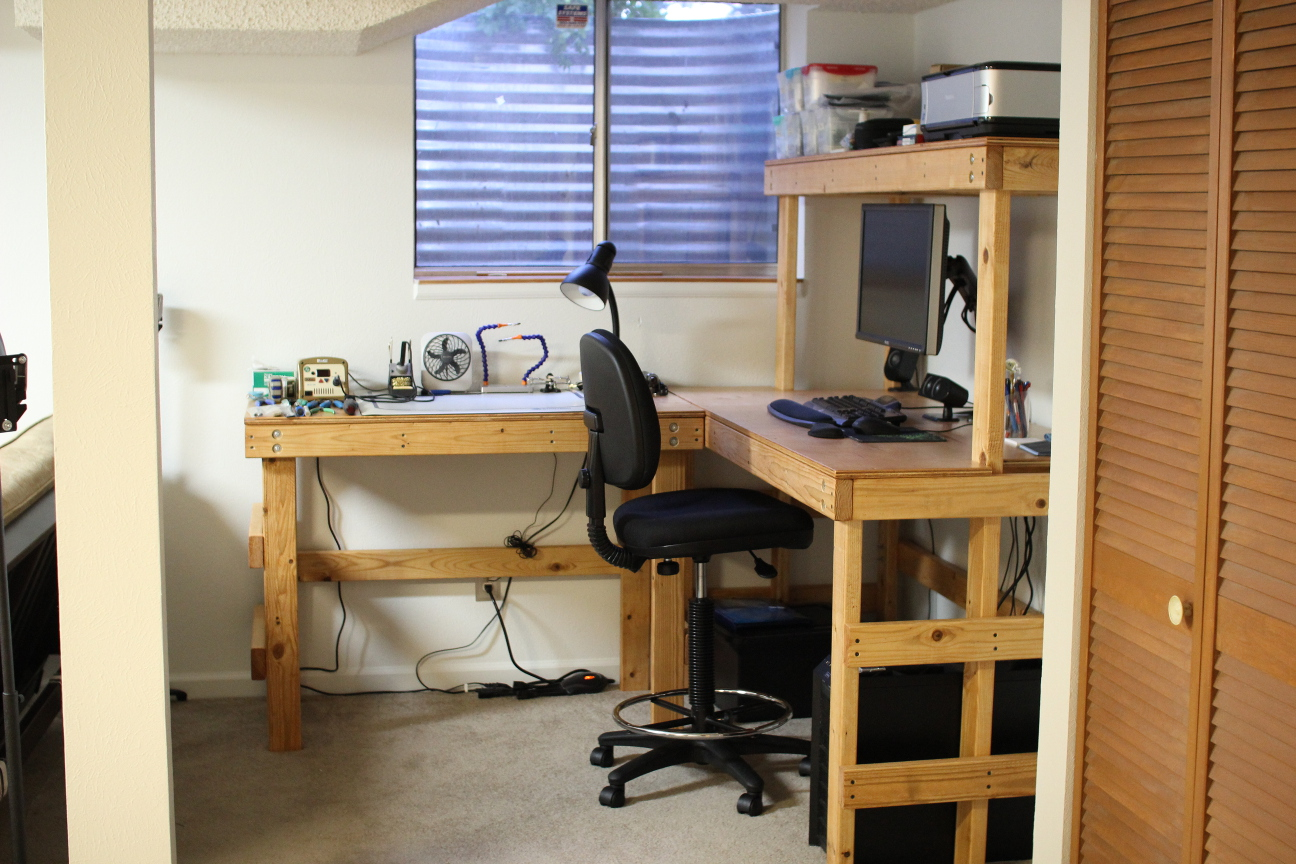
\includegraphics[height=0.2\textwidth]{bcollis/1wbench.jpeg}
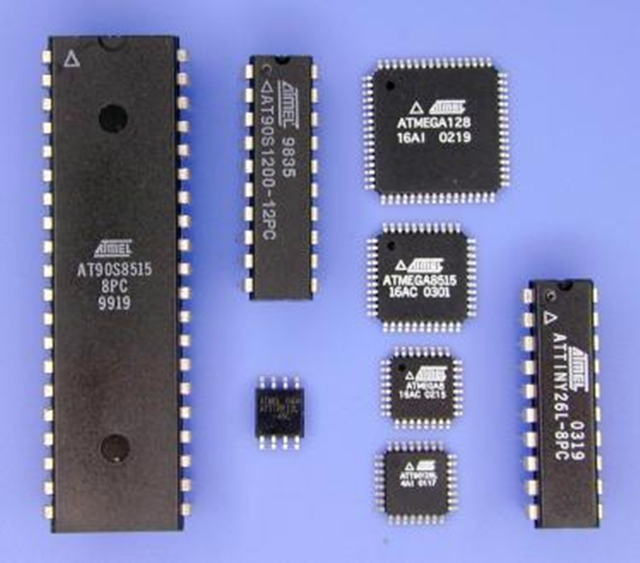
\includegraphics[height=0.2\textwidth]{bcollis/1atmels.jpeg}
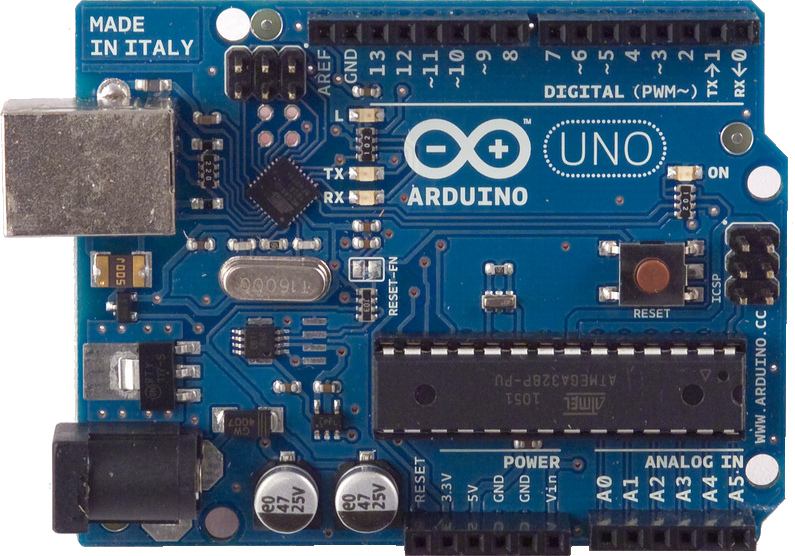
\includegraphics[height=0.2\textwidth]{bcollis/1arduino.jpeg}

\section{Ваше обучение по специальности <<Технология>>}

\subsection{Цели обучения технологиям Ново-Зеландской программы}

\begin{itemize}

\item \textbf{Технологическая практика}

\begin{itemize}

\item\textbf{Чоткость}: разработка ясных описаний для ваших технологических
проектов.

\item\textbf{Планирование}: думать прежде чем делать, и использовать во время
работы документацию: блок-схемы, принципиальные схемы, чертежи разводки плат,
диаграммы и эскизы.

\item\textbf{Наработка навыков}: сборка, отладка и тестирование электронных
схем, проектирование и изготовление печатных плат, написание программ для
микроконтроллеров.

\end{itemize}

\item \textbf{Технологические знания}

\begin{itemize}

\item\textbf{Моделирование}: прежде чем строить готовое электронное устройство,
сначала важно понять как оно работает путем моделирования и/или макетирования
аппаратного и программного обеспечения.

\item\textbf{Технологические продукты}: знания о компонентах и их
характеристиках.

\item\textbf{Технологические системы}: электронное устройство является более,
чем набором компонентов, это функционирующая система с входами, выходами и
контролирующим процессом.

\end{itemize}

\item \textbf{Природа технологии}

\begin{itemize}

\item\textbf{Значение технологических достижений}: знания об электронных
компонентах, особенно микроконтроллерах, как основе современных технологий.

\item\textbf{Роль технологии в обществе}: электронные устройства в настоящее
время играют центральную роль в инфраструктуре нашего современного общества;
подчинили ли они нас себе, как они изменили нашу жизнь?

\end{itemize}

\end{itemize}

\section{Ключевые компетенции Ново-Зеландской программы}

\begin{itemize}

\item\textbf{Знания}: для меня предметом технологии является все что относится к
знанию. Моя цель: заставить студентов понимать технологии, заложенные в
электронные устройства. Для достижения этого понимания студенты должны активно
учиться\note{в оригинале \textbf{enage}, англо-калька с \emph{себуанского}, NZ}\
в работе на самом раннем этапе, чтобы они могли построить собственное понимание
предмета и пойти дальше, чтобы стать хорошими решалами проблем. В начале
обучения электронике это требует от студентов восприимчивости к инструкциям,
которые им дают, и поиск ясности, когда они не понимают их.

Для этого на занятиях рассматриваются много новых и различных элементов знаний,
и студентам выдаются задания на решение проблем, чтобы помочь им мыслить
логически. Копирование чужого ответа наказывается, но приветствуется совместная
работа. В основе обучения лежит построение правильных концептуальных моделей и
анализ в контексте "большой картины".

\item\textbf{Взаимодействие}: работа в парах и группах, это важно как в классе,
так и в любой другой ситуации в жизни; мы все должны договариваться и разделять
ресурсы и оборудование с другими людьми; поэтому крайне важно активное общение и
помощь друг другу.

\item\textbf{Использование языка символов и текстов}: сердцем нашего предмета
является язык, который мы используем для обмена информацией в электронных
схемах, планах, алгоритмах и синтаксисе компьютерных языков программирования;
так что способность распознавать и правильно использовать символы и диаграммы для
работы, которую мы делаем, имеет критическое значение.

\item\textbf{Самоконтроль}: студенты принимают на себя личную ответственность за
собственное обучение; они принимают вызов, надеясь найти ответы в книгах или
найти учителя, способного объяснить им, что делать. Это значит, что студенты
должны взаимодействовать с рабочим материалом. 

Иногда ответы приходят легко, иногда нет; часто наша тема требует много проб и
ошибок (в основном ошибок). Студенты должны знать, что у них будут трудные
времена, пока не будет изучена б\'{о}льшая часть. И не сдаться в поиске
понимания.

\item\textbf{Участие и содействие}: мы живем в мире, который невероятно зависит
от технологии, особенно электроники; студенты должны развивать осознание
важности этой области человеческого творчества в нашей повседневной жизни, и
понимать, что наши проекты имеют и социальную функцию, а не только техническую.

\end{itemize}

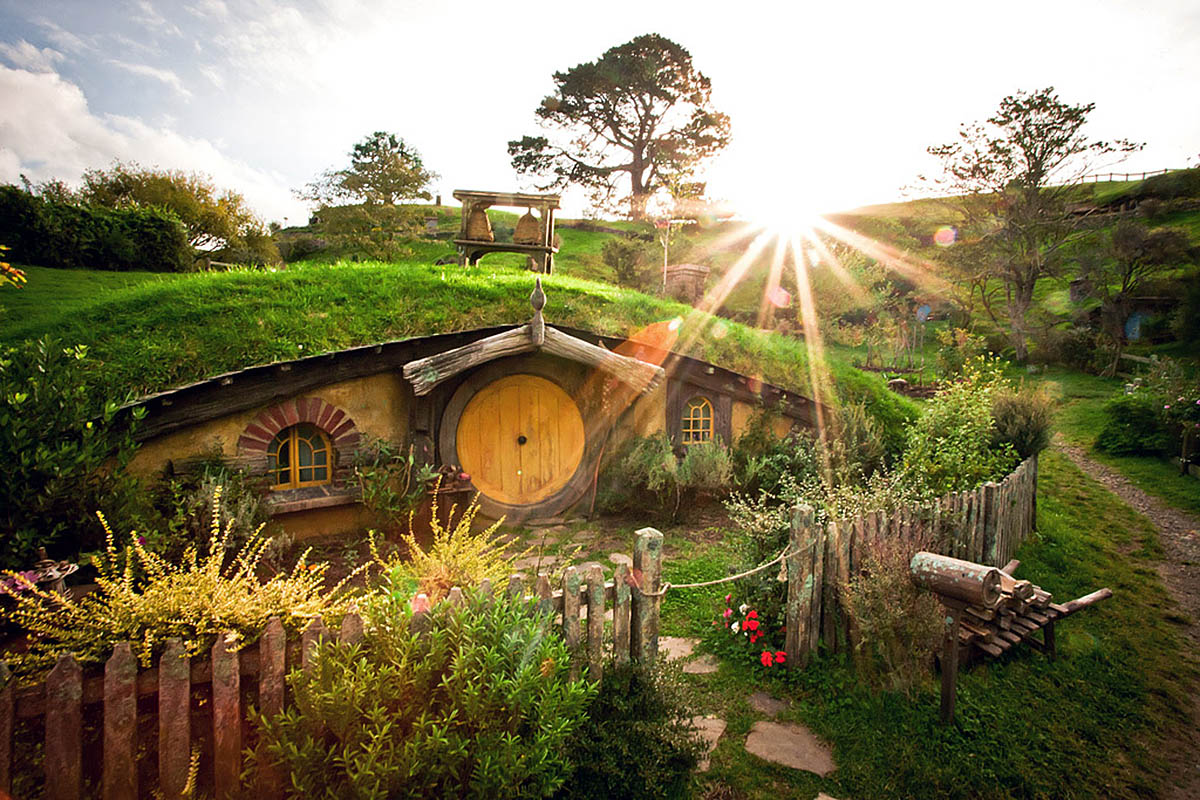
\includegraphics[height=0.95\textheight]{bcollis/12Hobbiton.jpeg}
